\section{Independent scope checks and source register}\label{app:scopechecks}

\subsection{The sign of compression}
For the forward branch $T_t=\sqrt{1+|\nabla T|^2}$, the characteristic velocity is minus the normalised gradient. In one dimension let $d=(1+T_0'^2)^{3/2}>0$. Then
\[
v_0'=-T_0''/d<0\quad\Longleftrightarrow\quad T_0''>0.
\]
This sign is independent of the density and reverses if the time branch is reversed. The scalar equivalence and the identity $1+(-1/\lambda)\lambda=0$ for $\lambda<0$ are separately checked in the analytic Lean supplement. These identities are not a formalisation of the full characteristic PDE theorem. For the periodic datum in Appendix~\ref{app:dust}, compactness ensures attainment. For a general noncompact datum, replacing a supremum by a maximum is an additional assumption.

\subsection{What an index can and cannot imply}
Write a signed index as $I=B-F$ with nonnegative integer counts. The toy example $B=3,F=2$ gives $I=1>0$ although fermionic states remain. Thus positivity cannot alone prove that every contributing state has zero angular momentum. Conversely, if assumptions $A_1,A_2,A_3$ imply $I>0$ and a computed index has $I<0$, one can conclude only $\neg(A_1\land A_2\land A_3)$. Selecting a particular failed assumption requires additional physics. This logical distinction is especially relevant when interpreting a negative full index as a statement about hair in every duality frame.

\subsection{The charge cone and reproducibility}
Equation (3.9) of \cite{Sen11positivity} contains $3(Q\cdot P)\le2Q^2+P^2$. The squared inner product occurs instead in the discriminant constraint. Mixing these two conditions changes the admissible charges. The Python scan uses the linear inequality, integer arithmetic, $Q^2\le12$, $P^2\le8$ and $Q\cdot P\le4$ and returns thirty negative triples. The Lean series certificate retains its original table range and verifies the original twenty-one triples with the corrected cone predicate. Its list is a subset, not an exhaustive scan of the larger box. The formal scope report records the exact toolchain, source hashes, successful checks and omissions.

\subsection{The base and the cover}
The local test $\chi=1$ already separates the two spaces. On the base, $\eta^2-h=0$ has derivative $\partial_h=-1$, hence is smooth. On the cover $h=\xi^2$, the equation becomes $(\eta-\xi)(\eta+\xi)=0$, a singular union at the origin. Blowing up or normalising the cover divisor may be useful for its invariants, but cannot turn this distinction into an error in the original weak-coupling expansion. The discriminant identity of Theorem~\ref{thm:senlimitk3} is checked as a polynomial identity in the analytic Lean supplement; the global geometry is not.

\begin{figure}[tbp]
\centering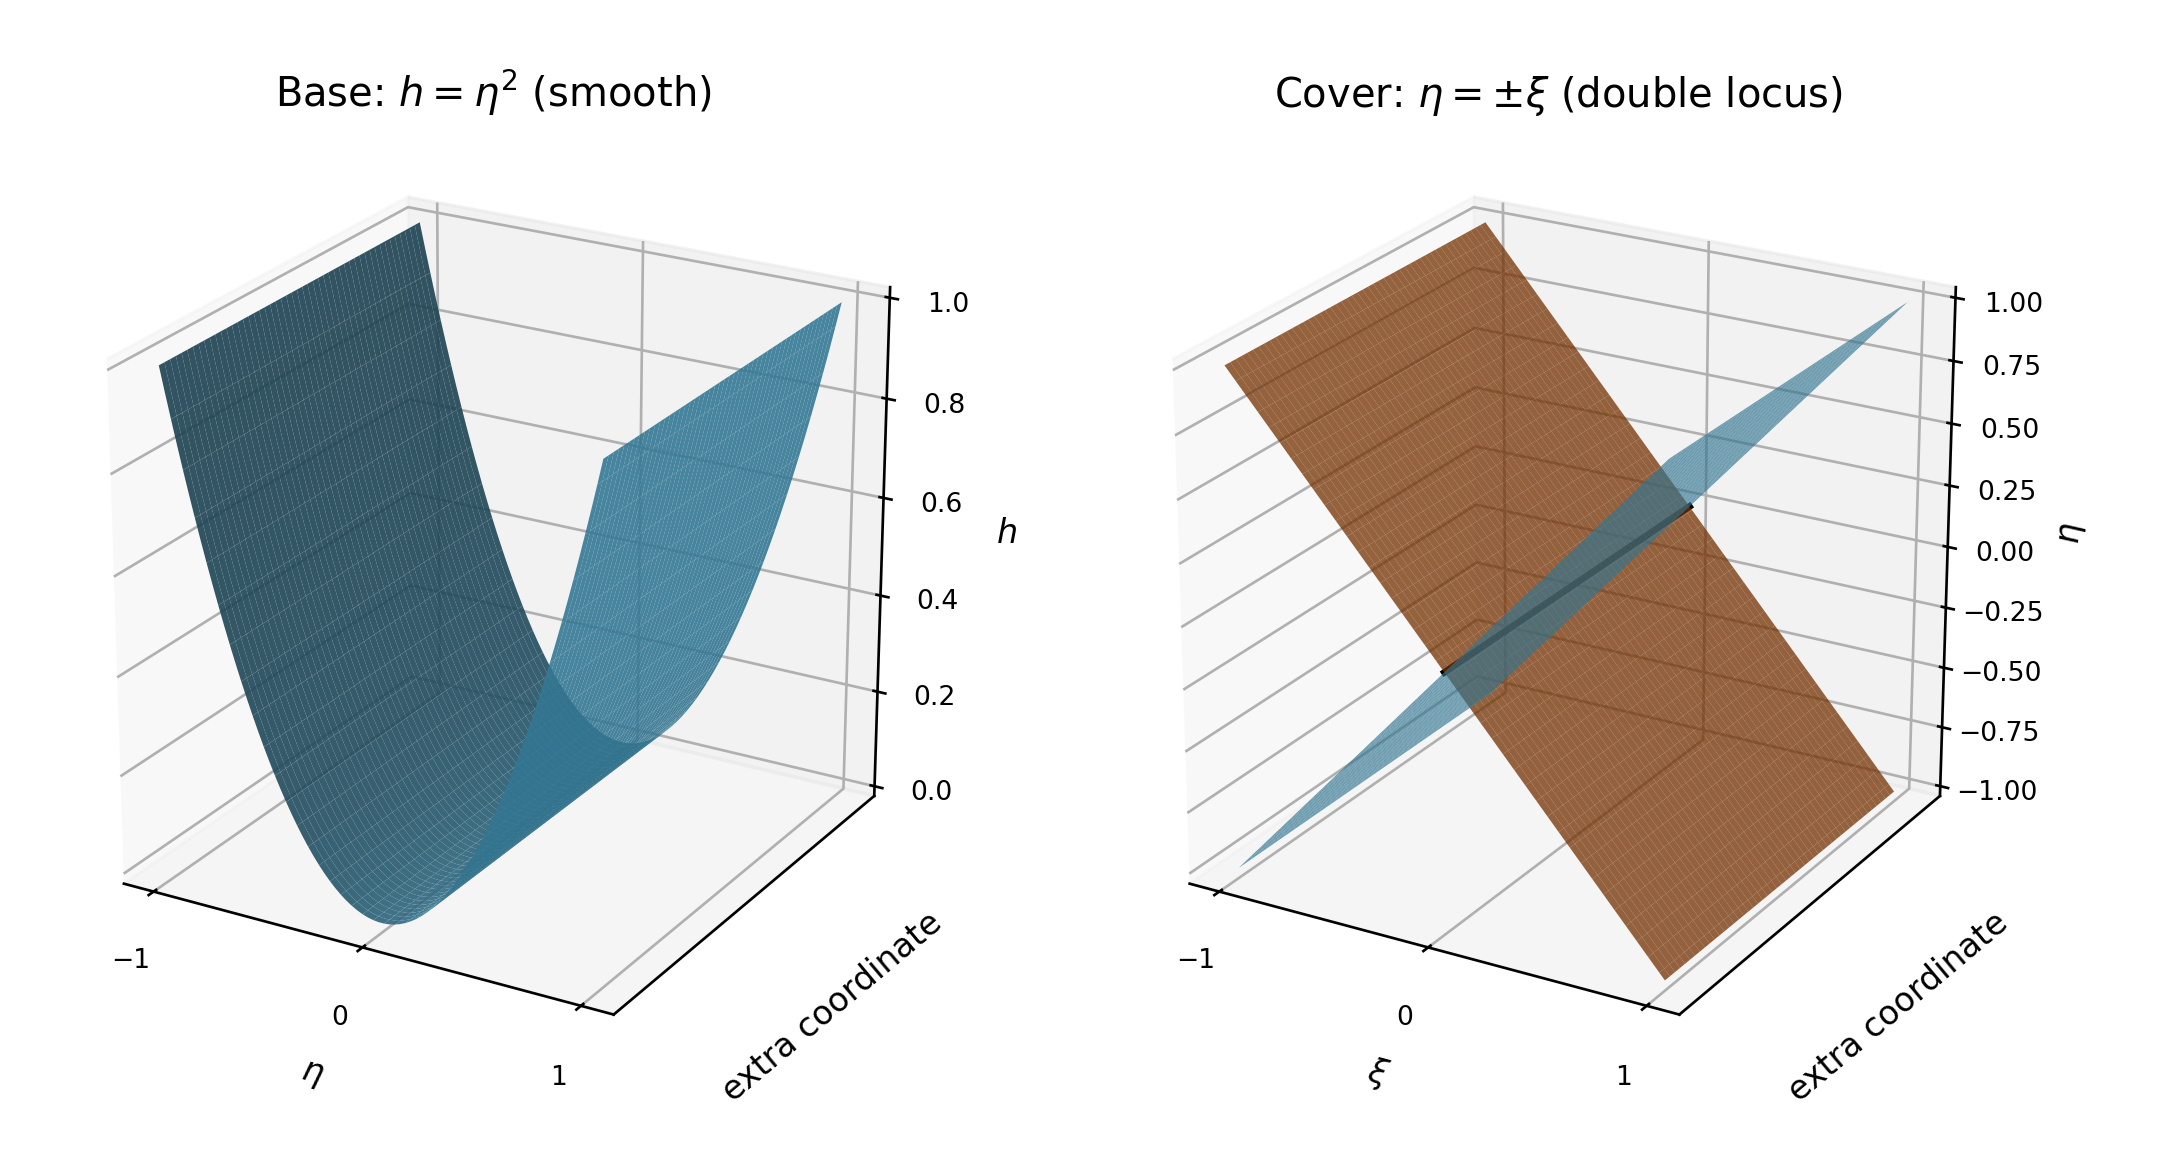
\includegraphics[width=0.94\linewidth,height=0.48\textheight,keepaspectratio]{figures/fig_base_cover.png}
\caption{Local distinction at $\chi=1$. The base divisor $h=\eta^2$ is smooth. Its pullback under $h=\xi^2$ consists of the crossing branches $\eta=\pm\xi$. The diagram displays real slices of complex divisors; it is a schematic, not a rendering of the full compactification.}
\label{fig:basecover}
\end{figure}

\subsection{Primary passages used for scope corrections}
The principal comparisons are reproducible from the following sources, with their original qualifications retained.
\begin{itemize}[leftmargin=1.4em,itemsep=2pt]
\item \cite{Sen11positivity}, introduction, pp.~3--5 and Eq.~(3.9): assumptions about hair and other index contributions, and the linear charge cone.
\item \cite{CD19}, Sections~4.1--4.2: known negative full indices in toroidal orbifolds; \cite{CD21}, Sections~4--5: proposed hair factors, finite positive horizon-index tests, and remaining mode-identification questions.
\item \cite{Sen02field}, Eqs.~(19)--(25): the pressureless Hamiltonian equations and the static solution with arbitrary density. The homogeneous decay assumption is stated in its abstract.
\item \cite{Sen97orientifold}, abstract, weak-coupling expansion and auxiliary double cover: the reduction is formal and singular auxiliary spaces are explicitly discussed. The D7 cover singularities are developed in \cite{CDE09}; global weak-coupling obstructions and the $I_0^*$ exception are in \cite{HLS18}.
\item \cite{Sen05stretching}, abstract and Gauss--Bonnet calculation: the higher-dimensional coefficient mismatch is reported by Sen, rather than discovered here.
\item \cite{Sen23localisation}: domain, ultraviolet and flat-direction issues are raised by Sen himself; they are not new unacknowledged objections.
\item \cite{KottkeRochon24}, Theorem~A: magnetic charge three is covered under the stated QFB-metric hypothesis. \cite{KrishnaSahoo23} separates proved one-loop universality from conjectural higher quantum extensions. \cite{KKMSS26} labels its beyond-Newtonian extension a conjecture.
\end{itemize}
This register is not evidence that every reference or every later citing paper has been independently checked. The bibliography supplies further context; new objections require their own exact source and hypothesis check.
